%%
% This is an Overleaf template for presentations
% using the TUM Corporate Desing https://www.tum.de/cd
%
% For further details on how to use the template, take a look at our
% GitLab repository and browse through our test documents
% https://gitlab.lrz.de/latex4ei/tum-templates.
%
% The tumbeamer class is based on the beamer class.
% If you need further customization please consult the beamer class guide
% https://ctan.org/pkg/beamer.
% Additional class options are passed down to the base class.
%
% If you encounter any bugs or undesired behaviour, please raise an issue
% in our GitLab repository
% https://gitlab.lrz.de/latex4ei/tum-templates/issues
% and provide a description and minimal working example of your problem.
%%

\documentclass[
  german,            % define the document language (english, german)
  aspectratio=169,    % define the aspect ratio (169, 43)
  % handout=2on1,       % create handout with multiple slides (2on1, 4on1)
  % partpage=false,     % insert page at beginning of parts (true, false)
  % sectionpage=true,   % insert page at beginning of sections (true, false)
]{tumbeamer}

 
% load additional packages

\usepackage{graphicx}
\usepackage{tikz}
\usepackage{url}
\usepackage{pgfplots}
\usepackage{hyperref}
\usepackage{pmboxdraw}
\usepackage{float}
\usepackage{babel}[ngerman]
\usepackage{csquotes}[autostyle]
\usepackage[useregional]{datetime2}
\usepackage{listings}
\usepackage{xurl}
\usepackage{enumerate}
\usepackage{circuitikz}
\usepackage{csquotes}
\usepackage{tikz-timing}
\usepackage{colortbl}
\usepackage{ifthen}
\usepackage{ulem}
\usepackage{pgf}

%\usepackage{minted}
%\usemintedstyle{borland}
\usetikzlibrary{patterns}
\pgfplotsset{compat=1.18}

% tikz
\usetikzlibrary{overlay-beamer-styles}
\usetikzlibrary{arrows,backgrounds,positioning,shapes,,patterns,patterns.meta,matrix,arrows,shapes.geometric}
\usetikzlibrary{matrix, fit}
\usetikzlibrary{automata}
% requires circuitikz >= 1.1.0
% for distros with older distributions, install TeX Live manually
% instead of using your package manager
% see: https://tug.org/texlive/quickinstall.html
\ctikzset{logic ports=european}

% minted

\lstset {
    frame=single,
    tabsize=4,
    breaklines=true,
    xleftmargin=5pt,
    xrightmargin=5pt,
    basicstyle=\ttfamily\footnotesize,
    %language=[RISC-V]Assembler,
}

\hypersetup { 
  colorlinks=true,
  urlcolor=blue,
  filecolor=black,
  linkcolor=black
}

% tikz  
\usetikzlibrary{fit}

% image path
\graphicspath{ {../resources/} }

% presentation metadata
\title{Übung 11: Pipelining}

\subtitle{Einführung in die Rechnerarchitektur}

\author{\theAuthorName}

\institute{\theGroupName\\\theSchoolName\\\theUniversityName}
\date{13. -- \DTMdisplaydate{2025}{01}{19}{-1}}

\footline{\insertauthor~|~\insertshorttitle~|~\insertshortdate}


% macro to configure the style of the presentation
\TUMbeamersetup{
  title page = TUM tower,         % style of the title page
  part page = TUM toc,            % style of part pages
  section page = TUM toc,         % style of section pages
  content page = TUM more space,  % style of normal content pages
  tower scale = 1.0,              % scaling factor of TUM tower (if used)
  headline = TUM threeliner,      % which variation of headline to use
  footline = TUM default,         % which variation of footline to use
  % configure on which pages headlines and footlines should be printed
  headline on = {title page},
  footline on = {every page, title page=false},
}


% available frame styles for title page, part page, and section page:
% TUM default, TUM tower, TUM centered,
% TUM blue default, TUM blue tower, TUM blue centered,
% TUM shaded default, TUM shaded tower, TUM shaded centered,
% TUM flags
%
% additional frame styles for part page and section page:
% TUM toc
%
% available frame styles for content pages:
% TUM default, TUM more space
%
% available headline options:
% TUM empty, TUM oneliner, TUM twoliner, TUM threeliner, TUM logothreeliner
%
% available footline options:
% TUM empty, TUM default, TUM infoline

\begin{document}

\maketitle

\begin{frame}[c]{Mitschriften \& Infos}{}
  \begin{minipage}[t]{\textwidth}
    \begin{columns}[c]
      \begin{column}{0.8\textwidth}
        Montags: \href{\zulipMo}{\zulipMo}
      \end{column}
      \begin{column}{0.2\textwidth}
        \includegraphics[width=0.8\linewidth]{\zulipMoQrFilename}
      \end{column}
    \end{columns}
  \end{minipage}
  \rule{\textwidth}{0.4pt}
  \begin{minipage}[t]{\textwidth}
    \begin{columns}[c]
      \begin{column}{0.8\textwidth}
        Donnerstags: \href{\zulipDo}{\zulipDo}
      \end{column}
      \begin{column}{0.2\textwidth}
        \includegraphics[width=0.8\linewidth]{\zulipDoQrFilename}
      \end{column}
    \end{columns}
  \end{minipage}
  \ifdefined\myWebsite
  \rule{\textwidth}{0.4pt}
  \centering
  Website: \href{\myWebsite}{\myWebsite}
  \fi
\end{frame}

\begin{frame}[c]{}{}
  \begin{center}
    \LARGE  Keine Garantie für die Richtigkeit der Tutorfolien.

    \Large Bei Unklarheiten/Unstimmigkeiten haben VL/ZÜ-Folien recht!
  \end{center}
\end{frame}

\begin{frame}[c]{Inhaltsübersicht}{}
  \begin{columns}[c]
    \begin{column}{1\textwidth}
      \begin{itemize}
        \item Quiz
        \item Wiederholung
        \item Tutorblatt
        \begin{itemize}
			\item Pipelining Speedup
			\item Flushen der Pipeline ohne Hazard Unit (Digital)
			\item Pipelining mit Hazard Unit
        \end{itemize}
      \end{itemize}
    \end{column}
  \end{columns}
\end{frame}

\begin{frame}[c]{Für die Klausur anmelden! (Frist: 15. Januar)}{}
	\begin{center}
		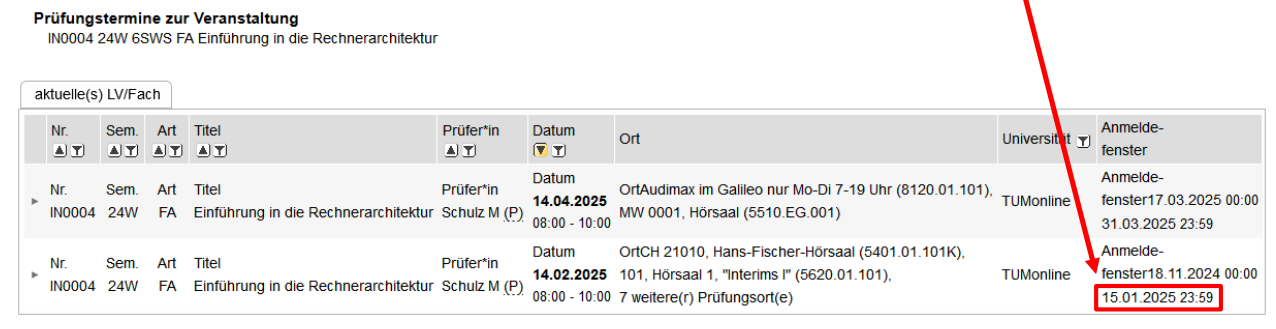
\includegraphics[width=\textwidth]{w11_klausuranmeldung.png}
	\end{center}
\end{frame}

\begin{frame}[fragile, c]{Pipelining}{}
	\begin{itemize}
		\item Parallele Verarbeitung von mehreren Instruktionen
		\item Aufteilung der Instruktionsverarbeitung in 5 Teilschritte: Fetch, Decode, Execute, Memory, Writeback
		\item Daten- und Kontrollpfad des Prozessors wird aufgeteilt: Register zur Zwischenspeicherung dazwischen
		\item maximaler Speedup: Anzahl $n$ der Pipelinestufen, Effekt bei großer Zahl an Instruktionen erkennbar
	\end{itemize}
\end{frame}

\begin{frame}[fragile, c]{Pipelining}{}
	\begin{center}
		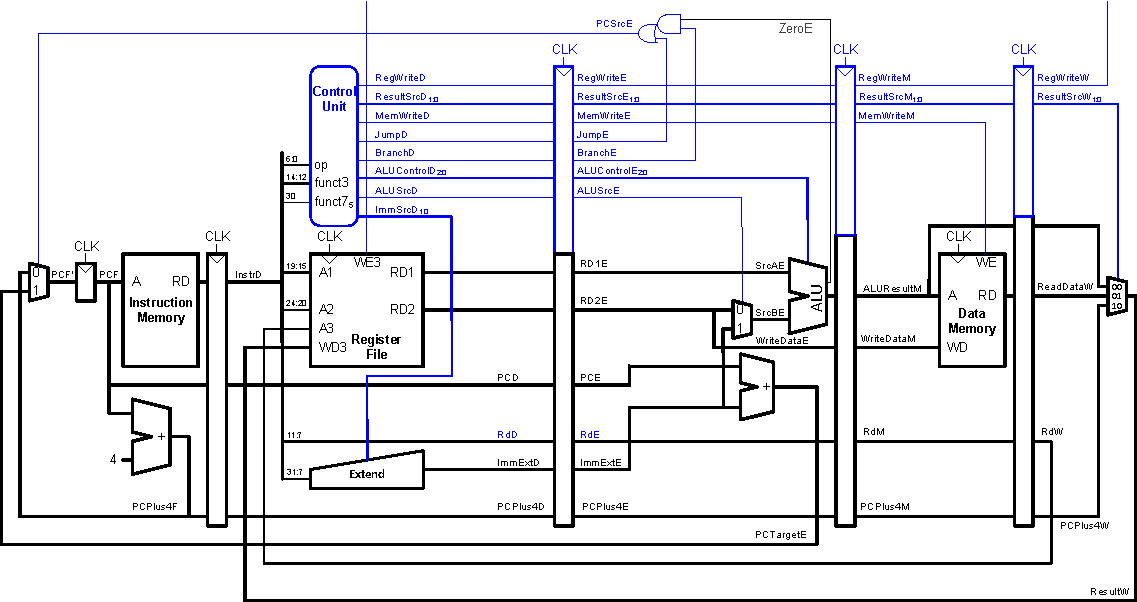
\includegraphics[width=0.85\textwidth]{w11_pipelined.pdf}
	\end{center}
\end{frame}

\begin{frame}[c, fragile]{Datenabhängigkeiten}{}
	\begin{columns}[c]
		\begin{column}{0.3\textwidth}
			{\ttfamily
				s1: lw {\only<1>{\color{red}}{t0}}, 0(a1)\\
				s2: lw t1, 0({\only<2>{\color{red}}{a0}})\\
				s3: add {\only<1>{\color{blue}}{t2}},  {\only<1>{\color{red}}{t0}}, s5\\
				s4: xor {\only<2,3>{\color{red}}{a0}},  {\only<1,2>{\color{blue}}{t2}}, a1\\
				s5: lw {\only<3>{\color{red}}{a0}}, 0(t1) \\
				s6: sub {\only<2>{\color{blue}}{t2}}, t3, t0  \\
			
		}
				\vspace{\baselineskip}\scriptsize{Mit * markierte Abhängigkeiten sind Datenkonflikte}

		\end{column}
		\begin{column}{0.4\textwidth}
			{\ttfamily
				\begin{tabular}{|c|c|c|c|c|c|}
					\hline
					i & F  & D  & E                                               & M                          & W                          \\
					\hline
					1 & s1 & -  & -                                               & -                          & -                          \\
					2 & s2 & s1 & -                                               & -                          & -                          \\
					3 & s3 & s2 & s1                                              & -                          & -                          \\
					4 & s4 & s3 & s2                                              & s1                         & -                          \\
					5 & s5 & s4 & \only<1>{\color{red}}{s3}                       & s2                         & \only<1>{\color{red}}{s1}  \\
					6 & s6 & s5 & \only<1>{\color{blue}}\only<2>{\color{red}}{s4} & \only<1>{\color{blue}}{s3} & \only<2>{\color{red}}{s2}  \\
					7 & ?  & s6 & \only<3>{\color{red}}{s5}                       & \only<3>{\color{red}}{s4}  & s3                         \\
					8 & ?  & ?  & \only<2>{\color{blue}}{s6}                      & s5                         & \only<2>{\color{blue}}{s4} \\
					\hline
				\end{tabular}
			}
		\end{column}
		\begin{column}{0.3\textwidth}
			\only<1,2>{Read after Write (RAW):
			{\ttfamily
			\begin{enumerate}[i.]
				\item s3, s1, t0*
				\item s4, s3, t2*
				\item s5, s2, t1
				\item s6, s1, t0
			\end{enumerate}
			}
			\vspace{\baselineskip}
			}
			\only<2,3>{Write after Read (WAR):
			{\ttfamily
			\begin{enumerate}[i.]
				\setcounter{enumi}{4}
				\item s4, s1, a1
				\item s4, s2, a0*
				\item s5, s2, a0
				\item s6, s4, t2*

			\end{enumerate}
			}
			\vspace{\baselineskip}
			}
			\only<3>{Write after Write (WAW):
			{\ttfamily
			\begin{enumerate}[i.]
				\setcounter{enumi}{8}
				\item s5, s4, a0*
				\item s6, s3, t2
			\end{enumerate}
			}
			}
		\end{column}
	\end{columns}
\end{frame}

\begin{frame}[c, fragile]{Datenkonflikte}{}
	\begin{itemize}
		\item Daten\textit{abhängigkeiten}: RAW, WAR, WAW
		\item Pipelinekonflikte: Datenkonflikte (data hazards) und Steuerkonflikte (control hazards)
		\item Daten\textit{konflikte} können nur bei RAW auftreten (müssen aber nicht): Abhängige Instruktion ist in der Execute-Phase, aber das Ergebnis wurde noch nicht zurückgeschrieben
		\item Steuerkonflikte treten bei Änderung der Kontrollflusses auf (branches, jumps)
	\end{itemize}
\end{frame}

\begin{frame}[c, fragile]{Lösung von Konflikten}
	Bei \textbf{data hazards} müssen mindestens \textbf{3 Befehle} zwischen zwei Instruktionen mit RAW-Abhängigkeit stehen:
	\begin{itemize}
		\item NOPs (Stalling)
		\item Befehlsumordnung (ohne Änderung der Semantik)
		\item Forwarding: noch nicht zurückgeschriebenes Ergebnis kann von der ALU direkt an den nächsten Befehl gegeben werden, falls dieser das Ergebnis benötigt
	\end{itemize}
	\vspace{0.5cm}
	Bei \textbf{control hazards} müssen mindestens \textbf{2 Befehle} zwischen der Sprungentscheidung und möglicherweise falsch geladenen Instruktion stehen.
	\begin{itemize}
		\item NOPs (Stalling)
		\item Branch Prediction (statisch/dynamisch): Falls Vorhersage falsch, müssen geladene Instruktionen entfernt werden
	\end{itemize}
	\vspace{0.5cm}
	weitere Konzepte: Out-of-Order-Execution, Register Renaming, \ldots
\end{frame}

\begin{frame}[c, fragile]{Forwarding}{}
	\begin{center}
		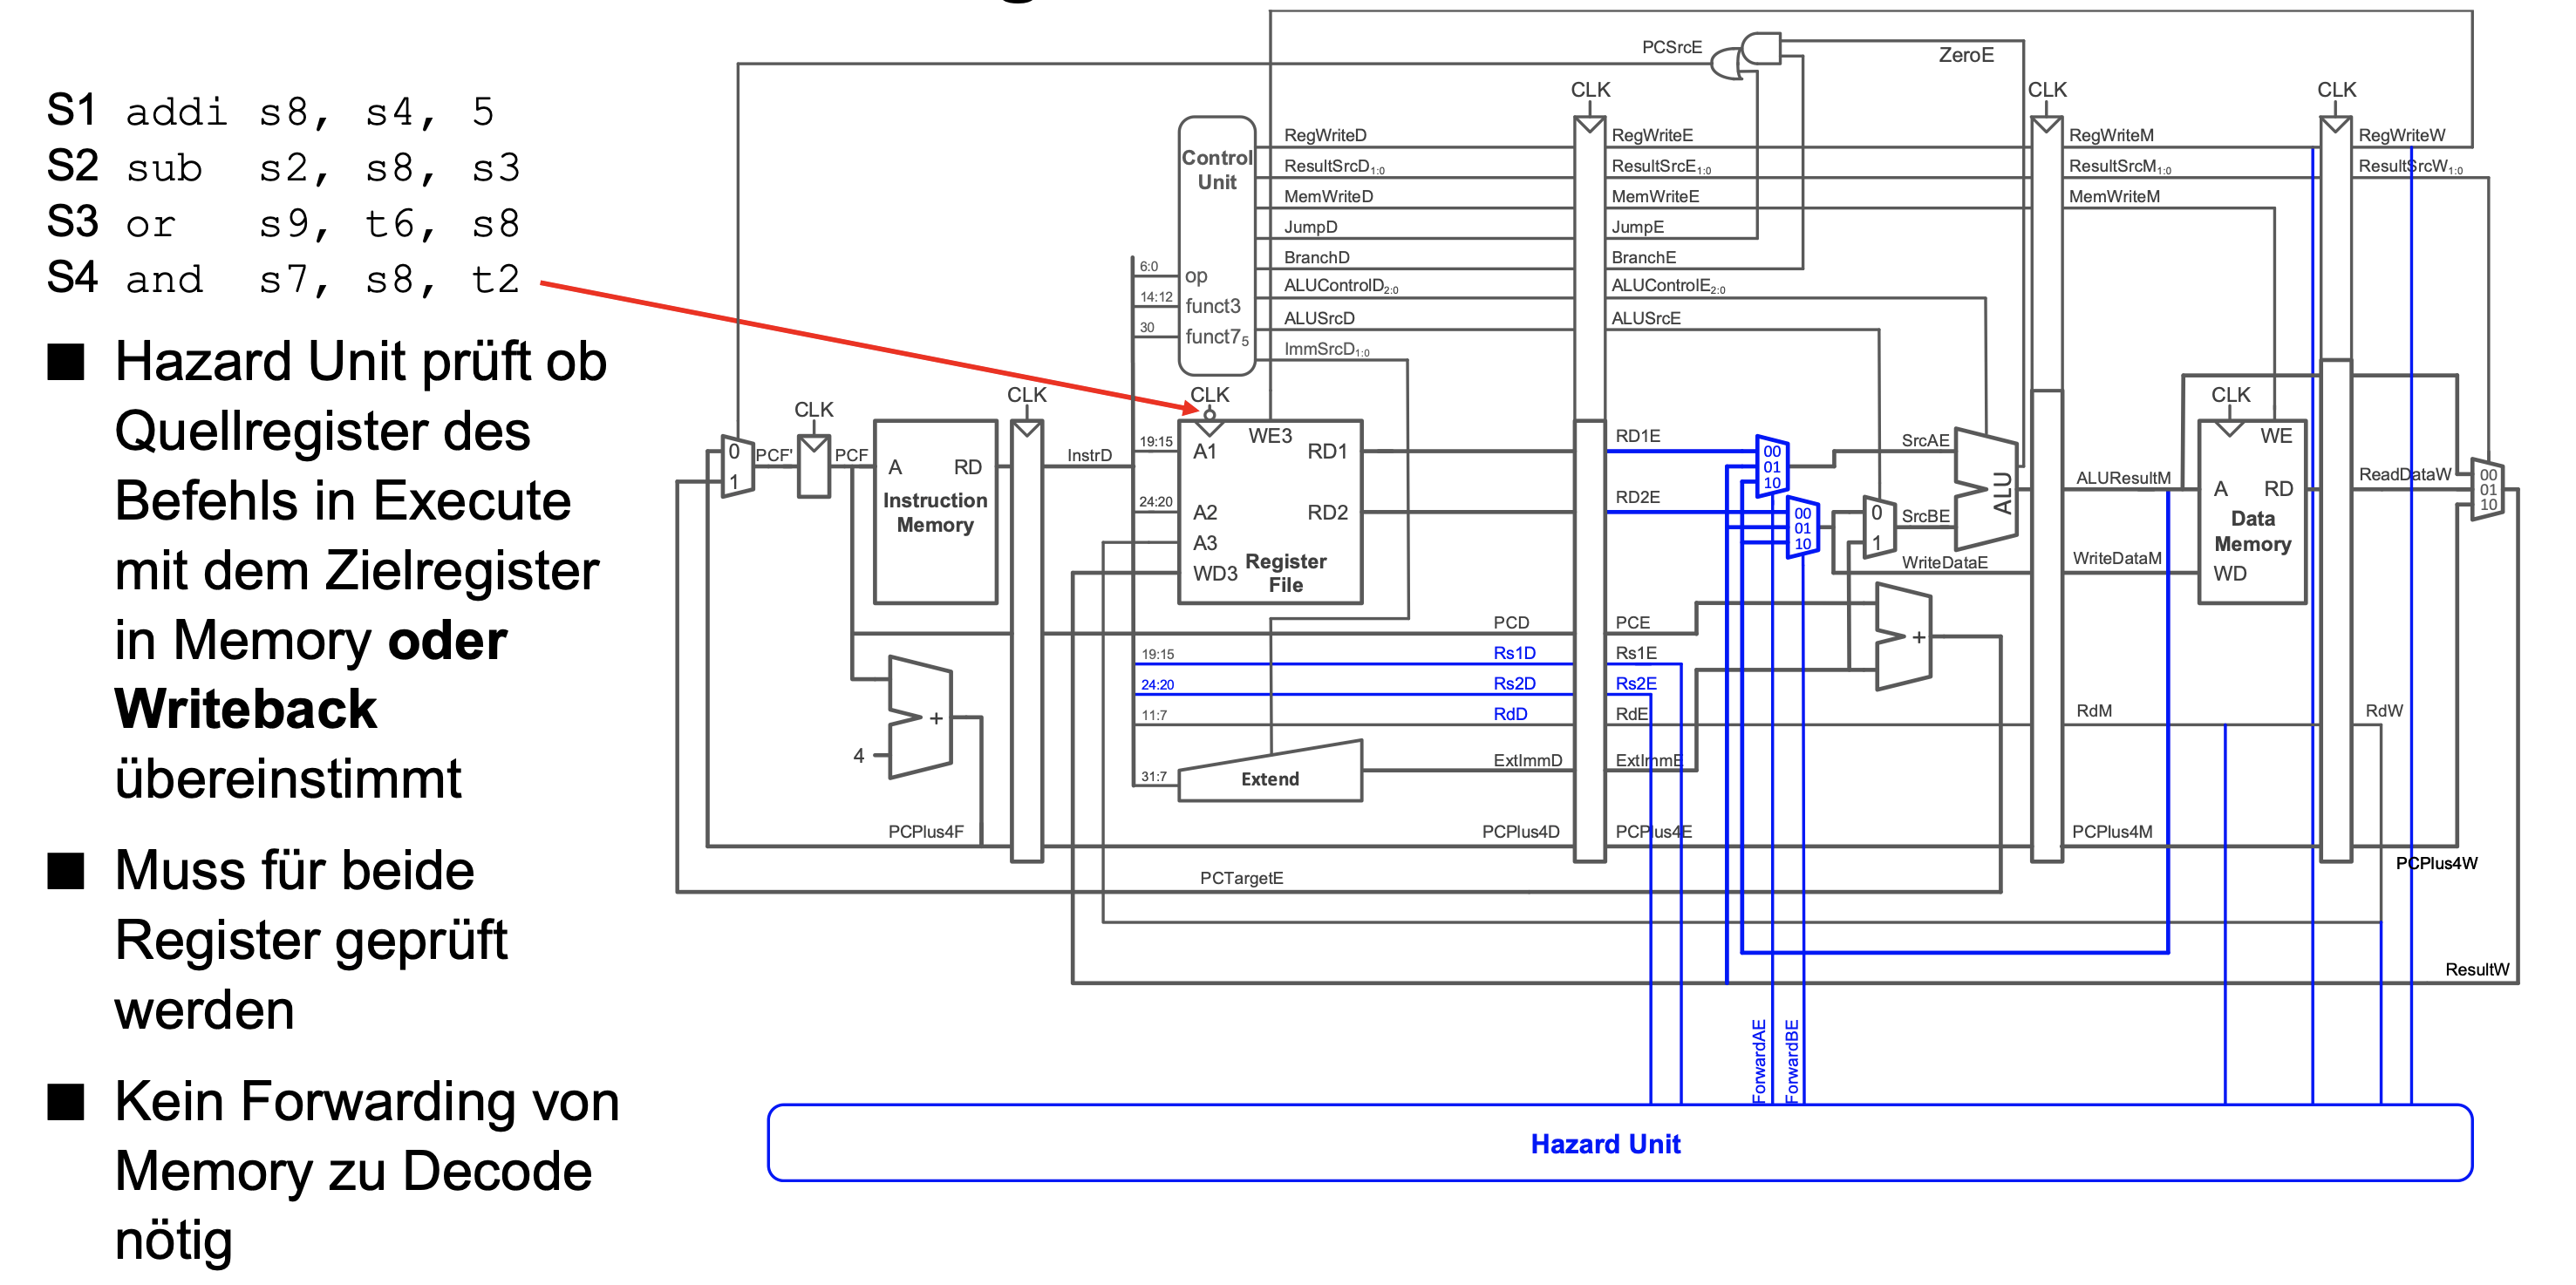
\includegraphics[width=0.9\textwidth]{w11_forwarding.png}		
	\end{center}
\end{frame}

\begin{frame}[c]{Feedback}{} 
  \begin{center}
    \includegraphics[width=0.30\textwidth]{\myFeedbackQrFilename}
  \end{center}
  \begin{center}
    \LARGE \href{\myFeedbackLink}{\myFeedbackLink}
  \end{center}
  \vspace{0.5cm}
  \begin{center}
    \small Ein Teil der Folien stammt aus dem Foliensatz von Niklas Ladurner. Vielen Dank dafür!
  \end{center}
\end{frame}

\end{document}